\documentclass[twoside, 10pt]{article}

\usepackage[T1, T2A]{fontenc}   % Standard package for selecting font encodings
\usepackage[utf8]{inputenc} % Accept different input encodings
\usepackage[ukrainian, english]{babel}

\usepackage{mathptmx}

\usepackage{indentfirst}    % Indent first paragraph after section header

\usepackage{sectsty}        % Control sectional headers
%\allsectionsfont{\mdseries\scshape\textbf}

\sectionfont{\normalfont\Large\textbf}
\subsectionfont{\normalfont\large\textbf}

\usepackage{multicol}       % Intermix single and multiple columns
\usepackage{orcidlink}      % Insert hyperlinked ORCiD logo
\usepackage{fancyhdr}       % Extensive control of page headers and footers

\usepackage{filecontents}
\usepackage{hyperref, doi}
\usepackage[numbers]{natbib}

\bibliographystyle{myunsrtnat}

% --- METADATA (ADJUSTED FOR NEW ARTICLE) ---
\def\myfirstpage{1}
\def\mylastpage{15}
\def\mypages{\myfirstpage-\mylastpage}
\def\myfilename{noether_casimir_drive_v2}
\def\myname{A. Drozdov}
\def\mynameukr{А. Дроздов}
\def\mytitle{Noether's Theorem and the Casimir Honeycomb Drive: On Non-Conservation of Momentum in Asymmetric Vacuum Systems}
\def\mytitleukr{Теорема Нетер та стильниковий рушій Казимира: про незбереження імпульсу в асиметричних вакуумних системах}
\def\myissn{2222-5617}
\def\mydoi{10.26565/2222-5617-2026-XX-XX} % ← placeholder, замените при подаче
\def\myemail{alexey.drozdov.07@gmail.com}
\def\ukrvisnyk{Вісник Харківського національного університету імені В.~Н.~Каразіна, серія «Фізика», вип. XX, \mypages~(2026)}
\def\envisnyk{The Journal of V.~N.~Karazin Kharkiv National University. Series “Physics” Iss. XX, \mypages~(2026)}
\def\myworkplace{V.~N.~Karazin Kharkiv National University, 61022, 4 Svoboda Sq., Kharkiv, Ukraine}
\def\myworkplaceukr{Харківський національний університет імені В.~Н.~Каразіна, майдан Свободи, 4, 61022 Харків, Україна}
\def\myorcidlink{0009-0004-1386-4534}

\def\myreceived{Received on January 9, 2026.}
\def\myaccepted{Accepted for publication on January 9, 2026.}
\def\myreceivedukr{Надійшла до редакції 9 січня 2026 р.}
\def\myacceptedukr{Прийнято до друку 9 січня 2026 р.}

\def\licenseref{http://creativecommons.org/licenses/by/4.0/}

\def\myvspacebeforesubsection{-2.0mm}
\def\myvspaceaftersubsection{-2.5mm}

\def\collontitulasfontcode{lmss}

\newcommand{\MyTitle}{\expandafter\MakeUppercase\expandafter{\mytitle}}
\newcommand{\MyTitleUkr}{\expandafter\MakeUppercase\expandafter{\mytitleukr}}

\fancypagestyle{firstpagestyle}{
% Definition of the header
\renewcommand{\headrulewidth}{0.6pt} % top horizontal rule
% Arial 9.5
\fancyhead[C]{\ukrvisnyk \\ \envisnyk}
\renewcommand{\footrulewidth}{0.6pt} % bottom horizontal rule
\fancyfoot[L]{\footbox{${}^{\copyright}$ \myname}}
\fancyfoot[R]{\footbox[r]{\fontencoding{T1}\fontfamily{\collontitulasfontcode}\selectfont \textit{Open Access. This article is licensed under a Creative Commons Attribution 4.0} \\
\href{\licenseref}{\textit{\licenseref}}}}
}

\usepackage{graphicx}
\usepackage{caption}
\DeclareCaptionFormat{nocaption}{}
\captionsetup{format=nocaption,aboveskip=0pt,belowskip=0pt}
\usepackage{float}
\floatplacement{figure}{H}
\usepackage{xcolor}
\usepackage{enumerate}
\usepackage{geometry}
\usepackage{amsmath, amssymb}
\usepackage{textcomp}
\usepackage{upquote}
\usepackage{ucs}
\usepackage{grffile}
\usepackage[Export]{adjustbox}
\adjustboxset{max size={0.9\linewidth}{0.9\paperheight}}
\usepackage{longtable, booktabs, enumitem, ulem, wrapfig, sidecap}

\providecommand{\keywords}[1]{\textbf{\textit{Keywords:}} #1}
\providecommand{\keywordsukr}[1]{\textbf{Ключові слова:} #1}

\author{\myname \,\orcidlink{\myorcidlink}}
\title{\textbf{\MyTitle.}}
\date{}

    % Colors for the hyperref package
\definecolor{urlcolor}{rgb}{0,.145,.698}
\definecolor{linkcolor}{rgb}{0,0,0}
\definecolor{citecolor}{rgb}{0,0,0}

\providecommand{\doi}[1]{DOI: \href{https://doi.org/#1}{#1}}

\geometry{verbose,a4paper,includehead,includefoot,
nomarginpar,
headheight=26pt,footskip=58pt,
tmargin=1.1cm,bmargin=1.0cm,lmargin=1.85cm,rmargin=1.85cm}
% Многострочные колонтитулы: \footbox выравнивает блок по нижней строке, поэтому он растёт
% вверх от базовой линии footskip и не уходит за край листа; footskip (58pt) больше высоты
% четырёх строк \scriptsize, поэтому текст на колонтитул не наезжает.
\newcommand{\footbox}[2][l]{\parbox[b]{0.88\linewidth}{\scriptsize\if#1r\raggedleft\else\raggedright\fi #2}}

\setlength{\columnsep}{0.5cm}

% forbid word transfer
\hyphenpenalty=10000

\begin{document}

\fontencoding{T2A}\fontfamily{ptm}\selectfont

\setcounter{page}{\myfirstpage}

% Set the page style to "fancy"...

\pagestyle{fancy}

%... then configure it.
\fancyhead{} % clear all header fields

% Arial 9.5
\fancyhead[CE]{\fontencoding{T1}\fontfamily{ptm}{\selectfont \textit{\mytitle.}}}

% Times New Roman 11
\fancyhead[CO]{\fontencoding{T1}\fontfamily{ptm}{\selectfont \textit{\myname}}}

\renewcommand{\headrulewidth}{0.6pt} % remove the top horizontal rule

\fancyfoot{} % clear all footer fields

% Arial 9.0
\fancyfoot[LE,RO]{\thepage}
\fancyfoot[LO]{\footbox{{\fontencoding{T1}\fontfamily{ptm}\selectfont \envisnyk} \\ {\fontencoding{T2A}\fontfamily{\collontitulasfontcode}\selectfont \ukrvisnyk}}}
\fancyfoot[RE]{\footbox[r]{{\fontencoding{T1}\fontfamily{ptm}\selectfont \envisnyk} \\ {\fontencoding{T2A}\fontfamily{\collontitulasfontcode}\selectfont \ukrvisnyk}}}
\fancyfoot[CO,CE]{}

$\,$


\thispagestyle{firstpagestyle}

\vspace{-9.4mm}

\fontencoding{T1}\fontfamily{ptm}\selectfont

\begin{tabular}{lcr}
\doi{\mydoi}
& \,\,\,\,\,\,\,\,\,\,\,\,\,\, \,\,\,\,\,\,\,\,\,\,\,\,\,\, \,\,\,\,\,\,\,\,\,\,\,\,\,\, \,\,\,\,\,\,\,\,\,\,\,\,\,\, \,\,\,\,\,\,\,\,\,\,\,\,\,\, \,\,\,\,\,\,\,\,\,\,\,\,\,\, \,\,\,\,\,\,\,\,\,\,\,\,\,\, \,\,\,\,\,\,\,\,\,\,\,\,\,\,
& ISSN \myissn (Print)
\end{tabular}

\vspace{9mm}

\begin{tabular}{l}
Original article \\
In print article \\
\href{https://doi.org/\mydoi}{https://doi.org/\mydoi} \\
UDC 53.09, 621.3, 629.7 \\
PACS numbers: 11.10.Ef, 03.70.+k, 42.50.Lc \\
\end{tabular}

\section*{\centering {\fontencoding{T1}\fontfamily{ptm}{\selectfont \MyTitle}}}

\vspace{7mm}
\centerline{\Large{\myname \,\orcidlink{\myorcidlink} }}
\vspace{7.5mm}
\centerline{\textit{\myworkplace}}
\centerline{\textit{E-mail: \href{mailto:\myemail}{\myemail}}}

\vspace{5mm}
\centerline{\myreceived}
\centerline{\myaccepted}

\vspace{5mm}

The Casimir honeycomb drive \cite{Drozdov2024} --- a perfectly conducting plate with a
nanoscale honeycomb structure on one side --- is examined from the standpoint of symmetries.
Because the vacuum modes on the two sides of the plate differ, the system is not invariant under
translations along the normal: the vacuum Hamiltonian depends explicitly on the coordinate \(l\),
and by Noether's theorem the field momentum along this axis is not conserved. The thrust equals
\(\partial\langle H\rangle/\partial l\). The same force is then computed independently, from the
Maxwell stress tensor built out of the fields of the cavity eigenmodes. Mode by mode the two
derivations coincide identically (Hellmann--Feynman theorem); after regularization they coincide
in the limit \(ak_m\to\infty\). Along the way an error in Appendix~B of \cite{Drozdov2024} is
found and corrected: for TM modes the ratio of pressure to energy density is \(k_z^2/k^2\), not
unity. The stress-tensor calculation shows where the force acts: it is the jump of
\(\langle T_{zz}\rangle\) at the metal surface, which is why the momentum flux through any closed
vacuum surface enclosing the plate is independent of the position of its faces. Finally, it is
shown that the standard momentum balance (Tamm, \S\,105) with \(\langle\mathbf S\rangle=0\) loses
exactly these jump terms. What is not conserved is the momentum of the field (and of the plate);
the total momentum of the system \emph{plate\,+\,field\,+\,support} is conserved.

\vspace{5mm}

\noindent
\begin{keywords}
\textit{Noether's theorem, Casimir effect, quantum vacuum, momentum non-conservation, Maxwell stress tensor, nanohoneycomb, Casimir thrust}
\end{keywords}

\vspace{5mm}

\fontencoding{T2A}\fontfamily{ptm}\selectfont

\noindent
\textbf{Як цитувати}: \textit{\mynameukr}. \textit{\mytitleukr}. {\ukrvisnyk}. \href{https://doi.org/\mydoi} {https://doi.org/\mydoi}.

\vspace{5mm}

\fontencoding{T1}\fontfamily{ptm}\selectfont

\noindent
\textbf{In cites}: \textit{\myname}. \textit{\mytitle}. {\envisnyk}. \href{https://doi.org/\mydoi} {https://doi.org/\mydoi}.

\vspace{5mm}

%\pagebreak
\newpage

\begin{multicols}{2}

\vspace{\myvspacebeforesubsection}
\subsection*{\centering{\fontencoding{T1}\fontfamily{ptm}{\selectfont INTRODUCTION}}}
\vspace{\myvspaceaftersubsection}


In \cite{Drozdov2024} it was shown that a perfectly conducting plate, one side of which is smooth
and the other covered with honeycomb cells of square cross-section \(a\times a\), experiences a net
force exerted by the electromagnetic vacuum. The force was computed as the difference of the
zero-point energy densities on the two sides of the plate, regularized by means of the
Euler--Maclaurin formula; for a cell size \(a\approx2\)~\(\mu\)m it turned out to be of the order of
several dynes per square metre.

Such a result inevitably raises a question: how is a one-body force compatible with momentum
conservation? In the classical two-plate Casimir configuration the forces on the plates are equal
and opposite, and the question does not arise. Here there is no second body.

The present paper answers this question in three steps.

\textit{The first step is symmetry.} Noether's theorem \cite{Noether1918} links momentum
conservation to translational invariance. The honeycomb plate breaks this invariance, so the field
momentum need not be conserved, and the force equals the derivative of the vacuum Hamiltonian with
respect to the plate position. This result coincides with the force of \cite{Drozdov2024}.

\textit{The second step is an independent check.} If the force is real, the Maxwell stress tensor
must give it as well. We build the tensor directly from the fields of the cavity eigenmodes and show
that for every mode the stress-tensor and Hamiltonian derivations coincide. This check revealed an
error in Appendix~B of \cite{Drozdov2024}, which we correct; it does not affect the Hamiltonian
result.

\textit{The third step is where the force acts and where the momentum goes.} The stress-tensor
calculation shows that the force is concentrated in the jump of the stress tensor at the metal
surface. The standard momentum balance equation (Tamm, \S\,105 \cite{Tamm1957}) contains no such
jumps; with a vanishing mean Poynting vector this is what creates the apparent paradox. We point out
the missing term and state precisely which momentum is not conserved.

All numerical statements of the paper are verified in the accompanying Jupyter notebook
\cite{VerifNotebook}.

\vspace{\myvspacebeforesubsection}
\subsection*{\centering{\fontencoding{T1}\fontfamily{ptm}{\selectfont STATEMENT OF THE PROBLEM}}}
\vspace{\myvspaceaftersubsection}


A plate of zero thickness lies in the plane \(z=0\) inside a cube \(L^3\) with perfectly conducting
walls (Fig.~1). On the side \(z>0\) the plate carries perfectly conducting cells of cross-section
\(a\times a\) whose walls reach the cube face \(z=l\) (in \cite{Drozdov2024} \(l=L/2\)). On the side
\(z<0\) there is the smooth face of the plate and a large cavity \(L\times L\times(L-l)\).

Each cavity is a rectangular resonator \(a\times b\times h\): for a cell \(a=b\), \(h=l\); for the
large cavity \(a=b=L\), \(h=L-l\). The wave numbers are \(k_x=\pi n_x/a\), \(k_y=\pi n_y/b\),
\(k_z=\pi n_z/h\); \(K^2=k_x^2+k_y^2\), \(k^2=K^2+k_z^2\), \(\omega=ck\). The notation
\(\sum_{n=(0)1}^{\infty}\) means that terms with \(n=0\) enter with weight \(\tfrac12\): each set
\((n_x,n_y,n_z)\) corresponds to two polarizations, but with one zero index only to one
\cite{Drozdov2024}.

\begin{figure}
\begin{center}
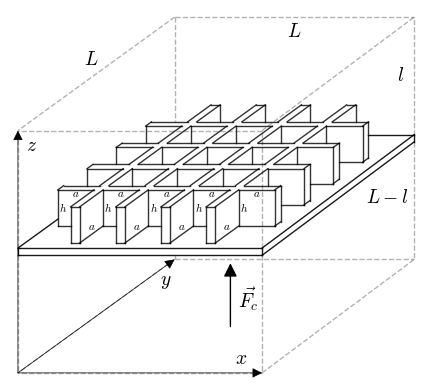
\includegraphics[width=0.42\textwidth]{honeycomb_box_H.png}
\caption{}{\centering{\textbf{Fig.1.} Cubic cavity with a plate covered by honeycomb.}}
\end{center}
\label{fig:honeycomb_box_H}
\end{figure}

The perfectly conducting walls of the cube, as in Casimir's work, are an auxiliary boundary
condition without a physical counterpart, similar to the periodic boundary conditions used in
quantum mechanics textbooks to normalize plane waves. The procedure is legitimate because the
result is taken in the limit \(L\to\infty\): by Weyl's theorem \cite{Weyl1912} the leading term of
the mode count, \(N(k)\simeq Vk^3/3\pi^2\), does not depend on the boundary conditions on the outer
faces, only surface corrections do, and the contribution of the remote walls to the force on the
plate vanishes. The cutoff \(k_m\) is a separate, physical element: it is set by the transparency of
the plate material to short waves.

\vspace{\myvspacebeforesubsection}
\subsection*{\centering{\fontencoding{T1}\fontfamily{ptm}{\selectfont NOETHER'S THEOREM AND NON-CONSERVATION OF MOMENTUM}}}
\vspace{\myvspaceaftersubsection}


The sum of zero-point energies \(E=\frac12\sum\hbar\omega\) over both cavities gives the vacuum
Hamiltonian per unit area \cite{Drozdov2024}:

\end{multicols}

\[
\frac{\langle 0|\hat{\mathcal{H}}|0\rangle}{S} = \frac{\hbar c}{a^2\pi} \Bigg\{
l \sum_{n_x=(0)1}^{\infty}\sum_{n_y=(0)1}^{\infty}
\int_0^{\infty} \sqrt{ \frac{\pi^2}{a^2}(n_x^2 + n_y^2) + k_z^2 } \, dk_z
+ (L - l) \int_0^{\infty}\!\!\int_0^{\infty}
\int_0^{\infty} \sqrt{k_x^2 + k_y^2 + k_z^2} \, dk_z \, \frac{a}{\pi}dk_x \frac{a}{\pi}dk_y
\Bigg\}.
\]

\begin{multicols}{2}

This expression depends explicitly on \(l\). Hence the system is \textbf{not invariant} under
infinitesimal translations of the plate \(z\to z+\delta z\).

By Noether's theorem the generator of spatial translations, the momentum component \(P_z\), is
conserved \textbf{if and only if} the Hamiltonian does not depend on \(z\). Since
\(\partial\langle H\rangle/\partial l\neq0\), the symmetry is broken, and \(P_z\) of the field is
not conserved. The net force is

\end{multicols}

\[
\frac{F}{S} = \frac{\partial}{\partial l} \frac{\langle 0|\hat{\mathcal{H}}|0\rangle}{S}
= \frac{\hbar c}{a^2\pi} \left\{
\sum_{n_x=(0)1}^{\infty}\sum_{n_y=(0)1}^{\infty}
\int_0^{\infty} \sqrt{ \frac{\pi^2}{a^2}(n_x^2 + n_y^2) + k_z^2 } \, dk_z
- \int_0^{\infty}\!\!\int_0^{\infty}
\int_0^{\infty} \sqrt{k_x^2 + k_y^2 + k_z^2} \, dk_z \, dn_x dn_y
\right\},
\]

\begin{multicols}{2}

which coincides with the thrust formula obtained in \cite{Drozdov2024} from the difference of energy
densities. After regularization by \(f(k/k_m)\) and two-dimensional Euler--Maclaurin summation it
takes the form \(F/S=\delta(E/V)=R(ak_m)\,\hbar c\,\pi/a^4\).

Thus the appearance of thrust is not unexpected: it is a direct consequence of the broken
translational symmetry. The quantum vacuum ``presses'' harder on one side because the mode spectra
on the two sides of the plate differ. Let us state at once which momentum is meant: it is the
translational symmetry of the \emph{boundary conditions}, not of space, that is broken. Therefore it
is the momentum of the field --- or, equivalently, of the plate that absorbs it --- that is not
conserved; the total momentum of the system \emph{plate\,+\,field\,+\,support} is conserved, just as
for an ordinary sail in the wind. Where exactly the field transfers momentum to the plate will be
shown by the stress tensor.

\vspace{\myvspacebeforesubsection}
\subsection*{\centering{\fontencoding{T1}\fontfamily{ptm}{\selectfont STRESS TENSOR FROM THE MODE FIELDS}}}
\vspace{\myvspaceaftersubsection}


Let us compute the force independently, through the Maxwell stress tensor, without assuming in
advance the momentum flux of a plane wave. Explicit fields of the TM and TE modes and the check of
Maxwell's equations and boundary conditions are given in Appendix~A. Gaussian units and Tamm's
notation \cite{Tamm1957} are used:
\(T_{ik}=\frac1{4\pi}(E_iE_k+H_iH_k)-\frac{\delta_{ik}}{8\pi}(E^2+H^2)\), the force on bodies
inside a closed surface is \(\oint T_{ik}n_k\,dS\), and the momentum flux is \(\Pi_{ik}=-T_{ik}\).
We need the component
\[
T_{zz}=\frac1{8\pi}\left(E_z^2+H_z^2-E_x^2-E_y^2-H_x^2-H_y^2\right),
\]
and denote the pressure on a horizontal area element by \(p\equiv-\langle T_{zz}\rangle\).

\textbf{Pressure of a single mode.} Average \(T_{zz}\) over the cross-section \(ab\) and over the
period. For \(n_x,n_y\ge1\) every factor \(\sin^2\) or \(\cos^2\) gives \(\tfrac12\), and for a TM
mode
\[
8\pi\langle T_{zz}\rangle=\frac{A^2}{8}\left[\cos^2k_zz\left(1-\frac{k^2}{K^2}\right)-\frac{k_z^2}{K^2}\sin^2k_zz\right]
=-\frac{A^2}{8}\frac{k_z^2}{K^2},
\]
since \(1-k^2/K^2=-k_z^2/K^2\). The energy density of the same mode averaged over the volume is
\(8\pi\overline w=\frac{A^2}{8}\frac{k^2}{K^2}\). Therefore
\[
p=-\langle T_{zz}\rangle=\overline w\,\frac{k_z^2}{k^2}.
\]
For a TE mode the same steps give the same result. If one of the transverse indices is zero
(possible only for TE), the overall factor doubles both in the pressure and in the energy, and the
ratio does not change; the TM mode with \(n_z=0\) has \(k_z=0\) and produces no pressure.

\textbf{Independence of \(z\).} The \(z\)-dependence has dropped out (\(\cos^2+\sin^2=1\)). The
general reason: in vacuum \(\partial T_{zk}/\partial x_k=\frac1{4\pi c}\,\partial_t[\mathbf E\times\mathbf H]_z\),
and the period average of a time derivative vanishes. On integrating over the cross-section, fluxes
through the side walls \(T_{zx}=\frac1{4\pi}(E_zE_x+H_zH_x)\) remain; on the walls \(x=0,a\)
\(E_z=0\) (tangential field) and \(H_x=0\) (normal field), i.e. \(T_{zx}=0\), and likewise
\(T_{zy}=0\) on \(y=0,b\). Hence \(\frac{d}{dz}\int\langle T_{zz}\rangle\,dx\,dy=0\). Note that only
the cross-section integral is independent of \(z\); at an individual point \((x,y)\) the value of
\(T_{zz}\) varies with \(z\), but it is the integral that enters the force. This fact will be used
in the next section.

\textbf{Sum over zero-point oscillations.} Each mode is an oscillator with energy \(\hbar\omega/2\)
in the ground state, shared equally between the electric and magnetic parts --- the same
distribution that the classical period average gives if one sets \(\overline w\,V=\hbar\omega/2\).
Therefore the pressure in a cavity is
\[
p=\frac{\hbar c}{2V}\sum_{\text{modes}}\frac{k_z^2}{k}.
\]
It differs from the energy sum \(E=\frac{\hbar c}{2}\sum k\) only by the summand: \(k_z^2/k\)
instead of \(k\).

\textbf{Identity with the Hamiltonian approach.} With \(k_z=\pi n_z/h\) we have
\(\partial k/\partial h=-k_z^2/(kh)\), and for every mode
\[
-\frac{\partial}{\partial h}\frac{\hbar ck}{2}=\frac{\hbar c}{2h}\frac{k_z^2}{k}=S\,p_{\text{mode}},\qquad V=Sh .
\]
The force found from the stress tensor coincides with \(-\partial E/\partial h\) mode by mode, even
before any regularization (the Hellmann--Feynman theorem \cite{Feynman1939}; in other words,
conservation of the adiabatic invariant \(E/\omega\) of each mode under a slow displacement of the
wall). The Hamiltonian force of the previous section is thereby confirmed by an independent method.

\textbf{Correction of Appendix~B of \cite{Drozdov2024}.} There the pressure on the \(xy\) face was
computed as \(\langle H_x^2+H_y^2\rangle/8\pi\). For TM modes this omits the term
\(-\langle E_z^2\rangle/8\pi\): with it the ratio of pressure to energy density equals
\(k_z^2/k^2\) for modes of both types, not \(1\) for the electric mode (for the mode \((2,1,3)\)
with \(a:b:h=1:1.3:2.7\) it is \(0.2119\) instead of \(1\)). Consequently the value \(1\) for the
electric mode and the inequality \(F/S\ge\delta(E/V)\) of \cite{Drozdov2024} that rests on it are
incorrect. The Hamiltonian derivation of Appendix~C is not affected: by the identity just proved it
coincides with the stress-tensor one mode by mode.

\textbf{Regularization.} With a cutoff \(f(k/k_m)\) the derivative of the mode energy is
\(-\partial_h\!\left[\frac{\hbar ck}{2}f\right]=\frac{\hbar c}{2h}\frac{k_z^2}{k}\left[f+\frac{k}{k_m}f'\right]\),
while the regularized stress-tensor sum \(\sum(k_z^2/k)f\) does not contain the second term. At
finite \(ak_m\) the two expressions therefore differ, but as \(ak_m\to\infty\) the difference
vanishes. For the honeycomb plate this is verified numerically (section ``Checks and estimates'').

\textbf{Symmetry check.} The renormalized electromagnetic tensor \(\langle T_{\mu\nu}\rangle\) is
traceless. Between two parallel plates the boundary conditions are invariant under boosts along the
plates; together with the trace condition this gives \(\langle\Pi_{zz}\rangle=3\langle u\rangle\)
(Brown and Maclay \cite{BrownMaclay1969}). A honeycomb cell is a waveguide along \(z\): far from its
ends its boundary conditions are invariant under boosts along \(z\), so in the \((t,z)\) block
\(\langle T_{\mu\nu}\rangle\propto\eta_{\mu\nu}\) and \(\langle\Pi_{zz}\rangle=-\langle u\rangle\),
i.e. \(|F/S|=\delta(E/V)\) --- the same value as the Hamiltonian approach gives. The argument is
exact for a perfect conductor in the limit \(ak_m\to\infty\) and up to end corrections of order
\(a/l\).

\vspace{\myvspacebeforesubsection}
\subsection*{\centering{\fontencoding{T1}\fontfamily{ptm}{\selectfont WHERE THE FORCE ACTS}}}
\vspace{\myvspaceaftersubsection}


\textbf{Jump at the metal surface.} At the face \(z=0\) (vacuum outside, inside the metal the fields
vanish) on the vacuum side \(E_x=E_y=0\), \(H_z=0\), while the normal \(\mathbf E\) and the
tangential \(\mathbf H\) jump by \(4\pi\sigma\) and \(\frac{4\pi}{c}\mathbf i\). Therefore
\[
T_{zz}\big|_{\text{vacuum}}=\frac1{8\pi}\left(E_z^2-H_x^2-H_y^2\right),\qquad
T_{zz}\big|_{\text{metal}}=0 .
\]
For a TM mode at \(z=0\) \(\langle E_z^2\rangle=\frac{A^2}{8}\),
\(\langle H_x^2+H_y^2\rangle=\frac{A^2}{8}\frac{k^2}{K^2}\), whence
\(-\langle T_{zz}\rangle(0^+)=\overline w\,k_z^2/k^2\) --- the same value as in the bulk of the
cavity; for a TE mode \(E_z=0\) and the result is the same. The jump
\([\![T_{zz}]\!]=T_{zz}|_{\text{metal}}-T_{zz}|_{\text{vacuum}}=p\) is the surface force per unit
area acting on the charges \(\sigma=E_n/4\pi\) in the field \(E_n\) and on the currents
\(\mathbf i=\frac{c}{4\pi}[\mathbf n\times\mathbf H]\) in the field \(\mathbf H_t\):
\[
\frac{f_z}{S}=\frac1{8\pi}\left(\langle H_t^2\rangle-\langle E_n^2\rangle\right).
\]
In the vacuum state \(\langle\sigma\rangle=0\) and \(\langle\mathbf i\rangle=0\), but the
correlations \(\langle\sigma E_n\rangle\) and \(\langle\mathbf i\times\mathbf H\rangle\) are
non-zero: the force is quadratic in the fields. For TE modes there is no surface charge on the
\(xy\) faces at all, and the jump is produced by the currents alone; this is an explicit example of a
jump of the tensor at a surface that carries no charge.

The plate has two such internal boundaries: the bottom of the cells and the smooth face. On each the
jump equals the pressure of the adjacent cavity,
\(p_{\text{cell}}=\frac{\hbar c}{2a^2l}\sum_{\text{cell}}\frac{k_z^2}{k}\) and
\(p_{\text{big}}=\frac{\hbar c}{2L^2(L-l)}\sum_{\text{big}}\frac{k_z^2}{k}\); inside the metal
\(T_{ik}=0\).

\begin{figure}
\begin{center}
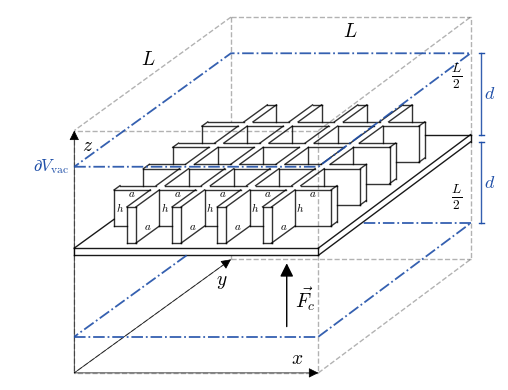
\includegraphics[width=0.42\textwidth]{honeycomb_box_L_d.png}
\caption{}{\centering{\textbf{Fig.2.} Faces of the pillbox \(\partial V_{\mathrm{vac}}\) at \(z=\pm d\).}}
\end{center}
\label{fig:honeycomb_box_L_d}
\end{figure}

\textbf{The pillbox.} Enclose the plate by a closed surface \(\partial V_{\mathrm{vac}}\) with faces
\(z=+d\) and \(z=-d'\) (\(0<d\le l\), \(0<d'\le L-l\)) spanning the whole cross-section
\(L\times L\) (Fig.~2); the side faces lie on the cube walls, where \(T_{zx}=T_{zy}=0\). Then
\[
\begin{aligned}
F_z&=\oint_{\partial V_{\mathrm{vac}}}\langle T_{zz}\rangle\,da
=\left[\langle T_{zz}\rangle(d)-\langle T_{zz}\rangle(-d')\right]L^2\\
&=(p_{\text{big}}-p_{\text{cell}})\,L^2 .
\end{aligned}
\]
By the proven independence of \(z\) the result does not depend on \(d\), \(d'\). For \(d,d'\to0\)
it is the sum of the two jumps at the plate faces --- the force acts on the metal surfaces; for
\(d=l\), \(d'=L-l\) the faces approach the auxiliary walls of the cube (for \(l=L/2\), the faces
\(z=\pm L/2\)), understood as a limit from inside the cavities. On the honeycomb side the face
crosses the cell walls; for perfectly conducting walls of zero thickness they do not contribute to
the integral. \(F_z>0\) (a push towards the cells) when \(p_{\text{big}}>p_{\text{cell}}\).

The flux through \(\partial V_{\mathrm{vac}}\) is the momentum flux of the \emph{field} through a
purely vacuum boundary, not a force applied directly to matter. It is non-zero only because the mode
spectrum, and hence \(\langle T_{zz}\rangle\), differs on the honeycomb side and on the smooth side.

\vspace{\myvspacebeforesubsection}
\subsection*{\centering{\fontencoding{T1}\fontfamily{ptm}{\selectfont WHY THE STANDARD MOMENTUM BALANCE DOES NOT SEE THIS}}}
\vspace{\myvspaceaftersubsection}


The standard momentum balance equation of the electrodynamics of continuous media (Tamm, \S\,105
\cite{Tamm1957}) reads

\end{multicols}
\[
\nabla\cdot\mathbf{T} = \frac{\partial\mathbf{g}}{\partial t} + \mathbf{f}_{\mathrm{vol}},
\qquad
\mathbf{g} = \frac{1}{c^2}\mathbf{S} = \frac{1}{4\pi c}[\mathbf{E}\times\mathbf{H}],
\]
\begin{multicols}{2}

where \(\mathbf{g}\) is the field momentum density and \(\mathbf{f}_{\mathrm{vol}}\) the density of
the volume ponderomotive force. For vacuum fluctuations of a static honeycomb system
\(\langle\mathbf{S}\rangle=0\), hence \(\langle\partial\mathbf{g}/\partial t\rangle=0\). If the field
momentum is identified with \(\mathbf g\), then with \(\langle\mathbf S\rangle=0\) there is no
momentum transport either --- and a one-body force seems impossible.

The transition from volume forces to stresses relies on Gauss's theorem, which Tamm applies
(\S\,33, Eq.~33.7) under the explicit condition that the tensor components be \emph{continuous}
inside the volume; surfaces of discontinuity are excluded there, and later (\S\,34, Eq.~34.8) only
their surface \emph{charges} are considered. But, as shown above, a vacuum--metal boundary may carry
no surface charge and still produce a finite jump of the stress tensor. This case is considered
neither in \S\,33 nor anywhere else in Tamm's book, including \S\,105. For a volume \(V\) containing
internal surfaces of discontinuity \(S_j\), Gauss's theorem must be written as

\end{multicols}
\[
\int_V \frac{\partial T_{ik}}{\partial x_k}\,dV
= \oint_{\partial V_{\mathrm{ext}}} T_{ik}\,n_k\,dS
\;-\; \sum_j \int_{S_j} [\![\,T_{ik}\,]\!]\,n_k\,dS_j ,
\]
\begin{multicols}{2}

where \([\![\cdot]\!]\) is the jump of a quantity across \(S_j\). The customary identification of
the field momentum with \(\mathbf{g}=\mathbf{S}/c^2\) keeps only the outer surface integral and loses
the jump terms. For the honeycomb plate it is precisely these terms that make up the whole force: the
sum of the two jumps at the plate faces equals the flux through the pillbox.

Two remarks make the interpretation unambiguous. First, as already stated, it is the momentum of the
\emph{field} (and of the plate absorbing it) that is not conserved, not the total momentum of a
closed laboratory system. Second, the renormalized vacuum stress \(\langle T_{\mu\nu}\rangle\) is a
physically measurable quantity --- it is the Casimir effect itself --- so the jump terms do not
require the assumption of a material ether: their value is fixed by the same
\(\langle T_{\mu\nu}\rangle\) that has been confirmed experimentally for the symmetric
configuration.

\vspace{\myvspacebeforesubsection}
\subsection*{\centering{\fontencoding{T1}\fontfamily{ptm}{\selectfont CHECKS AND ESTIMATES}}}
\vspace{\myvspaceaftersubsection}


\textbf{Two Casimir plates.} Plates at \(z=0\) and \(z=a\), outer cavities up to \(z=\pm L/2\). In
the gap \(k_z=\pi n/a\) and the transverse spectrum is continuous; per unit area (two polarizations)
\[
p_{\text{in}}=\frac{\hbar c}{a}\sum_{n\ge1}\int\frac{d^2k_\parallel}{(2\pi)^2}\frac{k_z^2}{k},
\]
and outside the sum over \(n\) is replaced by \(\frac a\pi\int dk_z\). By the independence of \(z\)
the value of \(p_{\text{in}}\) is the same in the middle of the gap and at the inner surface of each
plate, and \(p_{\text{out}}\) is the same at the outer surface and at the faces \(z=\pm L/2\). With
the cutoff \(e^{-k/k_m}\) the difference \(p_{\text{in}}-p_{\text{out}}\) equals \(-0.041043\),
\(-0.041110\), \(-0.041120\) in units of \(\hbar c/a^4\) for \(k_ma=20\), \(50\), \(100\) and tends
to \(-\pi^2/240=-0.041123\). The sign means attraction; with the Casimir energy density
\(u=-\pi^2\hbar c/720a^4\) this is the relation \(p=3u\) \cite{BrownMaclay1969}.

\textbf{Stress-tensor sum for the honeycomb.} For the honeycomb plate the stress-tensor sum
\(\sum k_z^2/k\) with the regulator \(f=1/(1+k^4/k_m^4)\) was computed by the same two-dimensional
summation as the energy sum in \cite{Drozdov2024}. Denote by \(D_E\) and \(D_T\) the energy and
stress-tensor ``sum minus integral'' differences. At small \(ak_m\) they differ even in sign (the
\(f'\) term), but at \(ak_m=9\) and \(14\) we obtain \(D_T+D_E=1\cdot10^{-4}\) and
\(4\cdot10^{-6}\), respectively, with \(|D_E|\approx0.012\): in the limit \(ak_m\to\infty\) the
stress-tensor and Hamiltonian derivations give the same force, \(|F/S|=\delta(E/V)\), in agreement
with the boost argument.

\textbf{Thrust estimate.} With \(\hbar c\,\pi/a^4=0.9932/a_\mu^4\)~dyn/cm\(^2\) (\(a_\mu\) is the
cell side in microns) the value \(R=0.0138\) from Table~1 of \cite{Drozdov2024} gives, for gold
honeycomb with \(a\approx2\)~\(\mu\)m, \(F/S\approx8.55\)~dyn/m\(^2\)
\(=8.55\times10^{-5}\)~N/m\(^2\). However, in \cite{Drozdov2024} the series over shells \(j\) was stopped as soon
as the current term fell below a threshold \(\epsilon\) (columns \(\epsilon\) and \(j_{max}\) of
Table~1). The tail terms are positive and decay as \(j^{-3}\), so the discarded remainder
\(\epsilon\,j_{max}^3\,\zeta(3,j_{max}+1)\approx\epsilon\,j_{max}/2\) is negligible at small \(ak_m\)
but reaches \(15\%\) at \(ak_m=9\) (\(j_{max}=99\)). With this correction Table~1 agrees with an
independent recalculation (closed form of the \(u\) integral, extrapolation in the size of the
summation domain) to within \(0.13\%\) in every row. The corrected limit \(|R|\approx0.0121\)
corresponds to \(F/S\approx7.5\)~dyn/m\(^2\). The order of magnitude and the conclusion about practical
applicability to satellite orbit correction are unchanged.

\vspace{\myvspacebeforesubsection}
\subsection*{\centering{\fontencoding{T1}\fontfamily{ptm}{\selectfont LIMITATIONS}}}
\vspace{\myvspaceaftersubsection}


(a) \textit{Cell height.} The calculation assumes that the cell walls reach the cube face and the
cell is a closed resonator. For real cells of height \(h\ll L\) the cell is open into the large
cavity, the modes do not separate, and this calculation does not describe such a case.

(b) \textit{Perfect conductor.} The jump is a property of a perfect conductor. In a real metal
\(T_{zz}\) decays to zero over the skin depth, and the integral of the force over the layer equals
the jump as long as the current in the metal is consistent with the field:
\(\mathbf j=\frac c{4\pi}\nabla\times\mathbf H\).

(c) \textit{Wall thickness.} Cell walls of finite thickness carry no \(z\)-force (\(T_{zx}=0\) on
them), but they reduce the fraction of the plate area occupied by the cavities.

(d) \textit{Regularization.} Which of the two regularized quantities --- energy or stress-tensor ---
is physical at finite \(ak_m\) cannot be decided within the model of a perfect conductor with a mode
cutoff; this requires a real \(\varepsilon(\omega)\), as in the method of Dzyaloshinskii, Lifshitz
and Pitaevskii \cite{DLP1961}, where the stress in a vacuum gap is found from the Green's function of
the field. For a honeycomb cell this requires the Green's function of a rectangular waveguide; this
is left for future work.

(e) \textit{Quantum average.} The equality of the electric and magnetic parts of the mode energy in
the ground state is used as a standard result for the oscillator and is not derived here.

\vspace{\myvspacebeforesubsection}
\subsection*{\centering{\fontencoding{T1}\fontfamily{ptm}{\selectfont CONCLUSION}}}
\vspace{\myvspaceaftersubsection}


The Casimir honeycomb drive is an example of a physical system in which Noether's theorem directly
explains the origin of a macroscopic force: \textbf{the absence of spatial homogeneity leads to
non-conservation of the field momentum}, and hence to thrust. An independent calculation through the
Maxwell stress tensor built from the mode fields reproduces the same force --- identically mode by
mode and, after regularization, in the limit \(ak_m\to\infty\) --- and corrects an error in
Appendix~B of \cite{Drozdov2024}. The stress-tensor calculation shows that the force acts on the
metal surfaces as a jump of \(\langle T_{zz}\rangle\), while the standard momentum balance of Tamm's
\S\,105, reduced to \(\mathbf g=\mathbf S/c^2\), does not contain these jump terms. The total
momentum of the system \emph{plate\,+\,field\,+\,support} is conserved. An experimental test of the
effect could confirm the link between the geometry of boundary conditions, symmetry and the dynamics
of the quantum vacuum.

\vspace{\myvspacebeforesubsection}
\subsection*{\centering{\fontencoding{T1}\fontfamily{ptm}{\selectfont APPENDIX A. MODE FIELDS}}}
\vspace{\myvspaceaftersubsection}


TM-mode fields (\(H_z=0\), \(n_x,n_y\ge1\), \(n_z\ge0\)):
\end{multicols}
\[
\begin{aligned}
E_z&=A\sin k_xx\,\sin k_yy\,\cos k_zz\,\cos\omega t, &
H_z&=0,\\
E_x&=-A\frac{k_xk_z}{K^2}\cos k_xx\,\sin k_yy\,\sin k_zz\,\cos\omega t, &
H_x&=-A\frac{k\,k_y}{K^2}\sin k_xx\,\cos k_yy\,\cos k_zz\,\sin\omega t,\\
E_y&=-A\frac{k_yk_z}{K^2}\sin k_xx\,\cos k_yy\,\sin k_zz\,\cos\omega t, &
H_y&=A\frac{k\,k_x}{K^2}\cos k_xx\,\sin k_yy\,\cos k_zz\,\sin\omega t.
\end{aligned}
\]
TE-mode fields (\(E_z=0\), \(n_z\ge1\), \((n_x,n_y)\ne(0,0)\)):
\[
\begin{aligned}
H_z&=A\cos k_xx\,\cos k_yy\,\sin k_zz\,\cos\omega t, &
E_z&=0,\\
H_x&=-A\frac{k_xk_z}{K^2}\sin k_xx\,\cos k_yy\,\cos k_zz\,\cos\omega t, &
E_x&=-A\frac{k\,k_y}{K^2}\cos k_xx\,\sin k_yy\,\sin k_zz\,\sin\omega t,\\
H_y&=-A\frac{k_yk_z}{K^2}\cos k_xx\,\sin k_yy\,\cos k_zz\,\cos\omega t, &
E_y&=A\frac{k\,k_x}{K^2}\sin k_xx\,\cos k_yy\,\sin k_zz\,\sin\omega t.
\end{aligned}
\]
\begin{multicols}{2}

Substitution verifies that \(\nabla\cdot\mathbf E=\nabla\cdot\mathbf H=0\),
\(\nabla\times\mathbf E=-\frac1c\partial_t\mathbf H\), \(\nabla\times\mathbf H=\frac1c\partial_t\mathbf E\)
for \(\omega=ck\), and that the perfect-conductor boundary conditions hold: tangential \(\mathbf E\)
and normal \(\mathbf H\) vanish on all six faces (on \(x=0,a\): \(E_y=E_z=0\), \(H_x=0\); on
\(y=0,b\): \(E_x=E_z=0\), \(H_y=0\); on \(z=0,h\): \(E_x=E_y=0\), \(H_z=0\)). These relations are
verified symbolically and numerically for the mode \((2,1,3)\) with \(a:b:h=1:1.3:2.7\).

For a TE mode, averaging over the cross-section and the period gives
\(\langle H_z^2\rangle=\frac{A^2}{8}\sin^2k_zz\),
\(\langle H_x^2+H_y^2\rangle=\frac{A^2}{8}\frac{k_z^2}{K^2}\cos^2k_zz\),
\(\langle E_x^2+E_y^2\rangle=\frac{A^2}{8}\frac{k^2}{K^2}\sin^2k_zz\), whence
\(8\pi\langle T_{zz}\rangle=-\frac{A^2}{8}\frac{k_z^2}{K^2}\) and \(p=\overline w\,k_z^2/k^2\).

\end{multicols}

\newpage

\fontencoding{T2A}\fontfamily{ptm}\selectfont

\section*{\centering {\fontencoding{T2A}\fontfamily{ptm}{\selectfont \uppercase{\MyTitleUkr}}}}

\centerline{\Large{\mynameukr \,\orcidlink{\myorcidlink} }}
\vspace{3mm}
\centerline{\textit{\myworkplaceukr}}
\centerline{\textit{E-mail: \href{mailto:\myemail}{\myemail}}}

\vspace{3mm}
\centerline{\myreceivedukr}
\centerline{\myacceptedukr}

\vspace{3.5mm}

Стільниковий рушій Казимира \cite{Drozdov2024} --- ідеально провідна пластина з нанорозмірною
стільниковою структурою з одного боку --- розглядається з погляду симетрій. Через асиметрію
вакуумних мод з двох боків пластини система не є інваріантною відносно трансляцій уздовж нормалі:
вакуумний гамільтоніан явно залежить від координати \(l\), і за теоремою Нетер імпульс поля вздовж
цієї осі не зберігається. Сила тяги дорівнює \(\partial\langle H\rangle/\partial l\). Потім ту саму
силу обчислено незалежно --- через тензор натягів Максвелла, побудований з полів власних мод
резонатора. Помодово обидва виведення збігаються тотожно (теорема Гельмана--Фейнмана), а після
регуляризації --- у границі \(ak_m\to\infty\). Попутно знайдено й виправлено помилку в додатку~B
роботи \cite{Drozdov2024}: для TM-мод відношення тиску до густини енергії дорівнює \(k_z^2/k^2\),
а не одиниці. Тензорний розрахунок показує, де прикладена сила: це стрибок \(\langle T_{zz}\rangle\)
на поверхні металу, і тому потік імпульсу через будь-яку замкнену вакуумну поверхню, що охоплює
пластину, не залежить від положення її граней. Нарешті, показано, що стандартний баланс імпульсу
(\S\,105 Тамма) при \(\langle\mathbf S\rangle=0\) втрачає саме ці стрибкові члени. Не зберігається
імпульс поля (і пластини); повний імпульс системи \emph{пластина\,+\,поле\,+\,опора} зберігається.

\vspace{3mm}

\noindent
\textbf{\textit{Ключові слова:}} \textit{теорема Нетер, ефект Казимира, квантовий вакуум, незбереження імпульсу, тензор натягів Максвелла, наностільники, тяга Казимира}

\begin{thebibliography}{9}
\bibitem{Drozdov2024}
A. Drozdov, \textit{Casimir honeycomb drive: on the force on perfectly conducting honeycomb on a plate}, The Journal of V. N. Karazin Kharkiv National University. Series “Physics”, Iss. 41, 28--41 (2024). \url{https://doi.org/10.26565/2222-5617-2024-41-04}
\bibitem{Noether1918}
E. Noether, \textit{Invariante Variationsprobleme}, Nachr. d. König. Gesellsch. d. Wiss. zu Göttingen, Math-phys. Klasse, 235–257 (1918).
\bibitem{Casimir1948}
H. B. G. Casimir, \textit{On the attraction between two perfectly conducting plates}, Proc. K. Ned. Akad. Wet. B \textbf{51}, 793 (1948).
\bibitem{Tamm1957}
I. E. Tamm, \textit{Fundamentals of the Theory of Electricity} (\S\,105, Maxwell stress tensor and the momentum balance of the electromagnetic field), Mir, Moscow (Engl.\ ed.\ 1979).
\bibitem{Feynman1939}
R. P. Feynman, \textit{Forces in molecules}, Phys. Rev. \textbf{56}, 340 (1939).
\bibitem{BrownMaclay1969}
L. S. Brown, G. J. Maclay, \textit{Vacuum stress between conducting plates: an image solution}, Phys. Rev. \textbf{184}, 1272 (1969).
\bibitem{Weyl1912}
H. Weyl, \textit{Das asymptotische Verteilungsgesetz der Eigenwerte linearer partieller Differentialgleichungen}, Math. Ann. \textbf{71}, 441 (1912).
\bibitem{DLP1961}
I. E. Dzyaloshinskii, E. M. Lifshitz, L. P. Pitaevskii, \textit{The general theory of van der Waals forces}, Sov. Phys. Usp. \textbf{4}, 153 (1961).
\bibitem{VerifNotebook}
A. Drozdov, \textit{Verification calculations for the paper ``Noether's theorem and the Casimir honeycomb drive''}, Jupyter notebook (SageMath 9.6), GitHub (2026). \url{https://github.com/daju1/articles/blob/master/casimir_noether/noether_casimir_verification.ipynb}
\end{thebibliography}

\end{document}
